\documentclass[12pt,a4paper]{article}
\usepackage[utf8]{inputenc}
\usepackage[T1]{fontenc}
\usepackage{amsmath}
\usepackage{textcomp}

\usepackage{geometry}
\geometry{a4paper,left=25mm,right=25mm, top=2cm, bottom=2cm} 

\usepackage{graphicx} %fuer bilder

\usepackage{verbatim}




 \usepackage{mathptmx}
 \usepackage[scaled=.90]{helvet}
 \usepackage{courier}



\usepackage{listings}
\usepackage{color}
 
\definecolor{dkgreen}{rgb}{0,0.6,0}
\definecolor{gray}{rgb}{0.5,0.5,0.5}
\definecolor{mauve}{rgb}{0.58,0,0.82}

\pagestyle{empty}
\lstset{numbers=left,language=C++}
\lstset{showstringspaces=false,
basicstyle=\ttfamily\footnotesize,
breaklines=true,
tabsize=3,
commentstyle=\color{dkgreen},      % comment style
inputencoding={ansinew},
title=\lstname %zeigt titel der datei an
}

\usepackage{pdfpages} % fuer pdfs
\usepackage{hyperref} % fuer url


%keine einrückungen bei absatz
\parindent 0pt

\begin{document}
\title{Übung 06}
\author{Reinhard Penn, Bernhard Selymes}
\date{April 2015}

\normalsize

%Beginn des Dokuments

\newcommand{\Uebung}{Random}
\newcommand{\srcpath}{../../src}
\newcommand{\simpath}{../../sim}

%Angabe
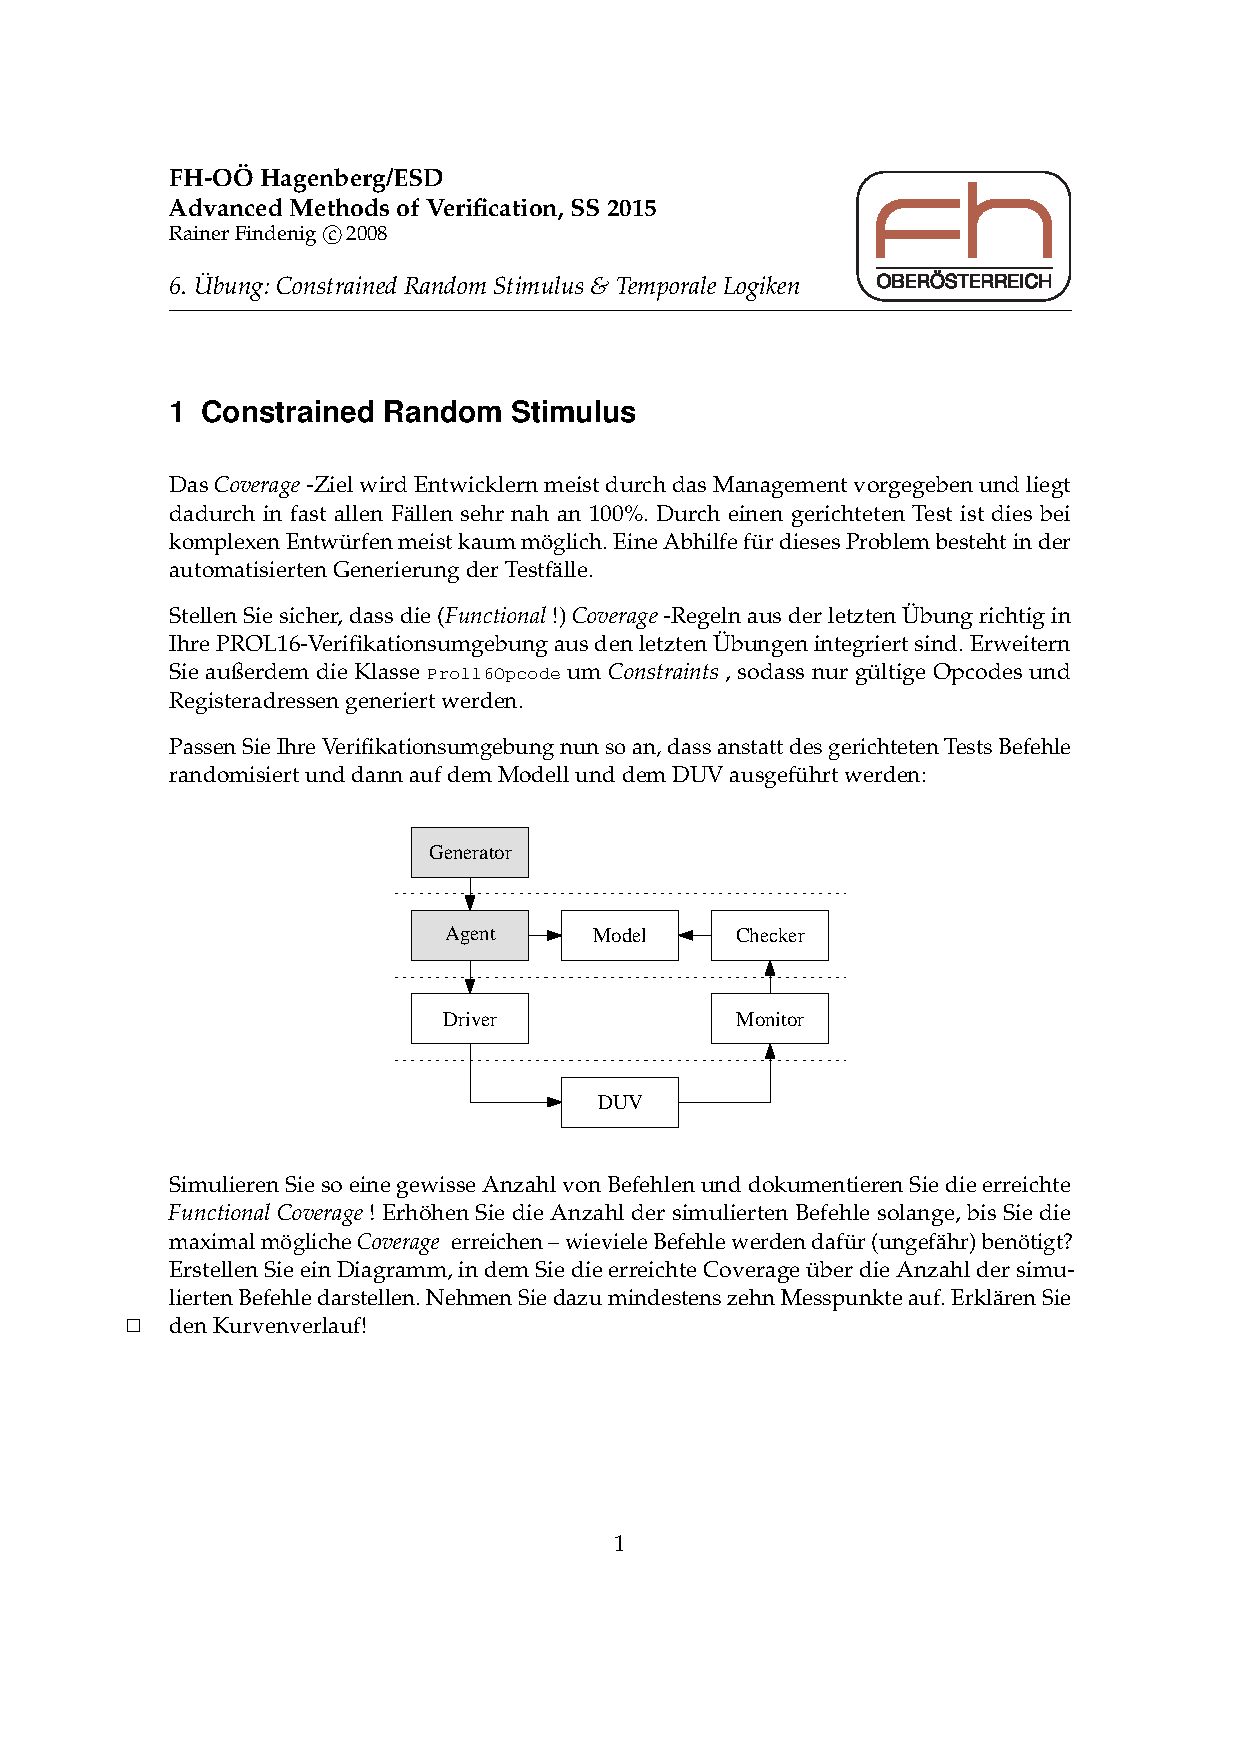
\includepdf[pages=-]{../Angabe.pdf}

\section{Beispiel 1}

\subsection{Diagramm}
%TODO


\subsection{Beantwortung der Fragen}

\begin{itemize}
	\item Randomisierte Werte sind nicht vorhersehbar. Es würden nur alle Fälle abgedeckt werden können, wenn unendlich viele Tests ausgeführt werden würden, was in der realen Welt nicht möglich ist.
	Bei vorhersehbaren Werten würde man sichergehen können, dass auch Cornercases getestet werden.
	\item Wurzelfunktion/Logarithmus (?). Je mehr Kombinationen ausgeführt werden desto geringer ist die Chance, dass eine Kombinationen ausgeführt wird, die noch nicht ausgeführt wurde.
	\item
				\begin{lstlisting}[numbers=none]
constraint ra_0 {
	ra dist { [0:0]:/50, [1:31]:/50 };
}
	
constraint rb_0 {
	rb dist { [0:0]:/50, [1:31]:/50 };
}

constraint nop_0 {
	(cmd == Nop) -> (ra == 0) && (rb == 0);
}
				\end{lstlisting}
		
	\item \texttt{randc} wiederholt Werte erst dann wenn alle ausgeschöpft wurden.
	\item Befehle: 21\\
				Befehle, die keine Flags beeinflussen: 6\\
				Befehle, die beide Flags beeinflussen: 11\\
				Befehle, Carry Flag 0 und Z Flag beeinflussen: 4\\
				
				Berechnung:\\
				keine Flags: 6 * 4 = 24
				Flags: 11 * 4 * 4 = 176
				Carry Flag 0: 4 * 4 * 2 = 32
				Summe: 232
				
				%TODO: Test aus der Übung Frage
\end{itemize}

\subsection{Source Code}

Der Sourcecode des Prol16 wurde nicht hinzugefügt, da der von der Elearning Plattform verwendet wurde.

\lstinputlisting[language={verilog}]{\srcpath/sv/ifProl16.sv}
\lstinputlisting[language={verilog}]{\srcpath/sv/pkgProl16.sv}
\lstinputlisting[language={verilog}]{\srcpath/sv/Prol16Command.sv}
\lstinputlisting[language={verilog}]{\srcpath/sv/Prol16Opcode.sv}
\lstinputlisting[language={verilog}]{\srcpath/sv/Prol16State.sv}
\lstinputlisting[language={verilog}]{\srcpath/sv/Prol16Model.sv}
%\lstinputlisting[language={verilog}]{\srcpath/sv/testProl16Model.sv}
\lstinputlisting[language={verilog}]{\srcpath/sv/testProl16Rand.sv}
\lstinputlisting[language={verilog}]{\srcpath/sv/top.sv}

\lstinputlisting[language={tcl}]{\simpath/CompileSimRandCov.do}

\subsection{Beispiel 2}

\end{document}
